\documentclass [french,12pt]{article}
\usepackage[french]{babel}
\usepackage[utf8]{inputenc} 
\usepackage{graphicx}
\usepackage{enumerate}
\title{Rapport de soutenance 1 \\Tartiflette}
\def\andcr{%
\end{tabular}%
\\
\begin{tabular}[t]{c}}
\author{ \andcr \andcr Rassoul Gabriel (rassou\_g) \andcr Chen Elliot (chen\_e) \andcr Habri Zakaria (habri\_z) \andcr Ozarowski Alexandre (ozarow\_a)}
\date{24 Octobre 2012}
\begin{document}
\maketitle
\clearpage
\tableofcontents
\clearpage
\section{Introduction}

“La reconnaissance optique de caractères (ROC, en anglais optical character recognition : OCR), ou encore appelé vidéocodage (traitement postal, chèque bancaire) désigne les procédés informatiques pour la traduction d'images de textes imprimés ou dactylographiés en fichiers de texte. Elle réalise beaucoup moins que l'être humain qui, lui, exécute, en plus de la reconnaissance, la compréhension du message, sa mémorisation, voire son analyse critique dans un seul temps.
\\
Un ordinateur réclame pour l'exécution de cette tâche un logiciel de ROC. Celui-ci permet de récupérer le texte dans l'image d'un texte imprimé et de le sauvegarder dans un fichier pouvant être exploité dans un traitement de texte pour enrichissement, et stocké dans une base de données ou du moins, sur un support sûr et exploitable par un système informatique.”
\\
Définition Wikipedia de Reconnaissance optique de caractères.
\\
OCR ou Optical Character Recognition qui signifie en français Reconnaissance de Caractères Optique est un logiciel capable de reconnaitre un texte dans une image et de le passer sous forme de texte éditable. Cela comprend l’effacement des traces résiduelles qui ne font pas parties du texte, la rotation de l’image pour qu’elle se retrouve parfaitement droite ainsi que la détection des blocs de textes et des caractères.
\\
C’est notre projet de Spé’Info à l’EPITA, qui est à réaliser en OCaml.
Pour cette première soutenance nous avons réalisé :
\\
La mise en niveaux de gris d’une image .
\\
L’effacement du bruit sur l’image.
\\
La binarisation de l’image
\\
La détecton de l’angle de redressement et la rotation de l’image.
\\
La détection des lignes de caractères dans l’image.
\\
La détection des caractères dans l’image.
\\
Egalement, nous utilisons un dépot git pour rassembler notre travail.
\\
\\
\section{Présentation de l'équipe}

\subsection{Zakaria Habri}

Originaire d’un couloir au milieu des montagnes marocaines, j’ai toujours vécuà Saint-Denis. Quand je ne fais pas de maths - car oui, j’aime les maths - j’aime jouer à des RPG assez matures, sur consoles portables, loin des FPS barbares ou adaptions identiques des mêmes jeux de sport. J’ai eu mon premier PC il y a 8 ans, quand j’avais 9 ans. Entre deux parties de Rayman, je l’explorais pour satisfaire ma curiosité: comment fonctionnait-il? Pourquoi ce trombone dansait-il ? Ma découverte de l’informatique est totalement due au hasard (il y a quelques années, taper ”devenir un hacker” sur Google renvoyait vers la page du tutoriel C du Site du Zéro !). Si mon niveau en programmation a été dopé par le projet de SUP, j'espère apprendre encore plus cette année en plongeant cette fois dans le monde merveilleux de Linux par l'intermédiaire du Caml.

\subsection{Ozarowski Alexandre}

J'ai commencé a m'intéresser à l'informatique à partir de la seconde à travers le sjeux vidéos. Cette année de SPE à l'école d'enseignement supérieure EPITA (école pour l'informatique et les techniques avancées) nous permet de créer un OCR. N'ayant jamais pensé au principe d'un OCR avant, ce projet me permet d'y penser et de participer à le créer. Ce qui rend ma motivation d'autant plus forte qu'après mon année de SUP, coder un projet est un plaisir et un puits de connaissance car ce on retient toujours mieux ce qu'on apprend par soi même que ce qu'on apprend par une tiers personne.

\subsection{}

\subsection{}

\section{Prétraitement de l'image}

\subsection{Matrices}

Pour traiter les images plus facilement dans cette partie nous avons choisies de d’appliquer chaque image à une matrice ou chaque élément de cette matrices sera représentatif d’un pixel avec sa valeur RGB.

\subsection{Niveau de gris}

La mise à niveau de gris va nous servir à mieux traiter l’image lors des prochaines étapes. Le but est de passer chaque pixel à une teinte entre noir et blanc.  La formule pour calculer le niveau de gris est la suivante :
	\\Gris = 0,299 * Rouge + 0,587 * Vert + 0,114 * Bleu
	\\Cette valeur remplace ainsi les trois champs RGB de chaque pixels. A partir de ce moment nous pouvons comparer deux pixels puisqu’ils ont tous les qu’une seule valeur pour les représenter.

\subsection{Effacement de bruit}

Le but de cette étape est éliminer toutes les petites imperfections de l’image pour que la reconnaissance de charactères se face plus facilement. Pour faire cette étape nous avons utilisé un filtre Gaussian. Nous allons nous baser sur les pixels autours de pixel étudier pour déterminer si sa couleur est la bonne où si il y’a eu une erreur lors de scan où si c’est une petite tache.\\
	L’algorithme marche de la manière suivante :\\
	Nous allons additionner la valeur des huit pixels autour de celui étudier avec la valeur de ce pixel. Chaque pixel a son propre coefficient en fonction de sa position. Ainsi les coefficients des pixels sur les coins est de un, il est faible car ils sont les plus éloigné. Les quatre autres pixels ont un coefficients de deux. Et le pixel étudier à un coefficient de quatre.\\
\\
\begin{center} 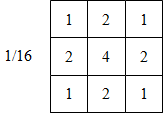
\includegraphics[scale=0.7]{Inline2.png} \end{center}.
\\
La somme des coefficients est de 16, nous allons donc diviser le résultat obtenu par 16 pour le rapporter à un nombre entre 0 et 255. Cette valeur est donc la nouvelle valeur de gris de pixel.
\\
	Il faut ensuite appliquer à cet algorithme pour chaque pixel et appliquer le résultats sur une nouvelle matrice pour éviter de contaminer le calcul des prochains pixels.

\subsection{Binarisation}

La binarisation consiste à passer l’image en noir et blanc. Pour obtenir un résultat plus net que de simplement vérifier si le pixel est au dessus ou en dessous de 127 (valeur moyenne) nous avons décidé de comparer la valeur du pixel à son seuil local. 
	\\Il y a plusieurs façon de calculer le seuil, la plus grosse différence est de choisir le nombre de pixel que nous voulons étudier. La méthode est plutôt simple, il suffit de parcourir tous les pixels autour de l’image et de ne garder que celui avec la plus faible valeur et celui avec la plus grande. On fait ensuite la somme des deux que l’on divise par deux et on compare le résultat au pixel étudié. Si le pixel a une plus grande valeur, on le passe en blanc, sinon on le met en noir.
 \\Nous avons longuement hésité entre prendre les 8 pixels autours du pixel étudié ou de prendre les 49. Après avoir comparé les résultats sur de nombreuses images nous avons décidé d’utiliser 8 pixels parce que cela nous donna de meilleurs résultats sur des images avec une plus faible dimension.
\\
\\
\section{Détection d'angle et rotation}

Tout d'abord, pour aborder la rotation d'un document scanné qui est penché d'un certain angle, il faut préciser que ce travail va se faire en deux étapes. 
\\En premier temps, il y a la détection de l'angle de rotation pour pouvoir redressé le document. Pour ce faire on a implémenté la transformée de Hough, inventée par Paul Hough en 1962 pour la reconnaissance des formes dans le traitement d'image. Même si celle ci malheureusement, ne donne pas encore les bonnes valeurs.
Le principe de cette algorithme a été dure a appréhender et comprendre. En effet peu de documents en parlent sur internet, certes il existe des livres, des œuvres sur cette algorithme, mais ceux ci étaient trop long pour être abordé avant la soutenance.
\\
Principe :\\
	On suppose que notre image a été pré-traité et que c’est une image binaire.
\\
Hough fait une remarque :
\\
Il existe un nombre infini de droites passant par un unique point. Et la seule chose qui les différencie est leur orientation.
Le but de cette transformée étant de déterminer lesquelles de ces droites passent au plus près de l’image attendu. Dans la transformée de Hough chaque ligne correspond à un vecteur de coordonnées paramétriques (theta,rho) avec theta l’angle de notre pente et rho la norme du vecteur (la longueur du segment perpendiculaire à la droite d'angle theta et passant par l'origine). Ainsi en calculant toutes les valeurs de rho pour chaque angle theta pour un point donné, on obtient une sinusoïde appelée espace de Hough. Si les sinusoïdes de deux points se coupent, alors on obtient les paramètres rho et theta caractéristiques de la droite passant par ces deux points. On a donc l’angle d’inclinaison de notre ligne de texte.


\begin{center} 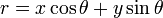
\includegraphics[scale=0.8]{r.png} \end{center}.
\\
\begin{center} 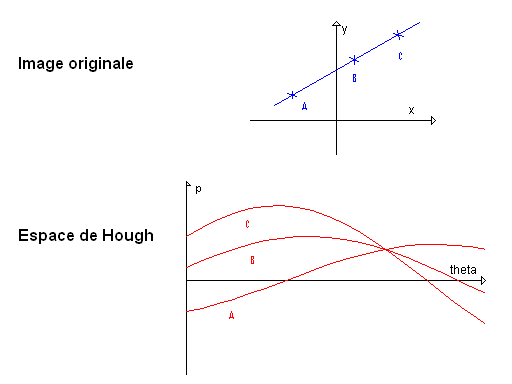
\includegraphics[scale=0.7]{Hough_sample2.png} \end{center}.
\\

Concrétement, on crée une matrice dite de “vote” où l’on déterminera combien de points passent par tel ou tel angle theta. Ensuite on parcours notre image, et pour chaque pixel noir, on va dans un premier temps définir theta, que l’on fera varier dans une grosse plage d’angle. Puis on calcule rho, s’il est positif on rajoute 1 au vote de coordonnées (theta, rho) dans la matrice de vote, sinon on ne le prend pas en compte. Et au moment où l’on ajoute un vote, on enregistre le vote le plus grand rencontré. On se retrouve donc à la fin avec l’angle le plus probable à  utiliser pour la rotation pour obtenir un texte horizontale.
\\
\\
\\
\section{Détection des Caractères}
\subsection{Détection des blocs de texte}

La détection des zones de texte utilise trois procédés :
\\
\\
Le remplissage horizontal :
\\
            Il s'agit de créer une nouvelle image à partir de l'image binarisée. On parcourt l'image (de haut en bas, puis de gauche à droite) en recopiant les pixels tel quel sur l'image d'arrivée s'ils sont blanc. En revanche, si un pixel est noir on stocke son abscisse dans une variable "minimum" et on continue de parcourir la ligne en stockant les abscisses des pixels noirs dans une variable "maximum". Ainsi, en fin de ligne, on peut "écrire" des pixels noirs sur l'image d'arrivée à l'ordonnée courante et en partant de l'abscisse "minimum", à l'abscisse "maximum", ce qui aura pour effet de tracer une ligne de pixels noirs sur toute la longueur de la ligne de texte. On remet "minimum" et "maximum" à 0 et c'est parti pour le prochain tour de boucle !
\\
	Le résultat final sera une image composée de blocs de longueurs internes inégales, ce problème va être corrigé grâce au remplissage vertical.
\\
Le remplissage vertical :
\\
            La méthode est fondamentalement identique à l'horizontale. On parcourt l'image, de gauche à droite, puis de haut en bas, cette fois, et on recopie les pixels blancs. Quand on rencontre un pixel, on stocke son ordonnée comme "minimum" et on continue de parcourir la colonne en stockant les ordonnées des pixels noirs dans une variable "maximum". En fin de colonne on trace une ligne de pixels noirs sur l'image d'arrivée de "minimum" à "maximum", ce qui correspond aux lignes contenant du texte. 
\\
            Le résultat final en lui même est inutilisable (un gribouillis de lignes verticales, voilà ce que c'est !), mais en le "fusionnant" avec le résultat du remplissage horizontal la détection de blocs sera optimale.
\\
La fusion :
\\
           Le mot fusion est bien joli, mais on applique en réalité un ET logique entre les images résultantes des remplissages.
           Pour cela on parcourt les deux images en même temps :
\\
                    si les pixels courant sont de même couleur, on garde cette couleur,
                    sinon, on met le pixel courant de l'image résultant en blanc.
\\
Le résultat final est une image composée uniquement de blocs noirs représentant les zones de texte.

\subsection{Détection des caractères (des lettres)}

Cette détection utilise deux procédés.
\\
Détection des lettres en tant qu' ensemble de pixels noirs adjacents :
\\
        Il s'agit d'étudier le tracé de chaque lettre pour les délimiter. Pour ce faire, on parcourt la matrice de l'image d'origine, et lorsqu'on rencontre un pixel noir, on le remplace par la valeur k, puis on part en récursion sur les pixels adjacents : s'il sont noirs, on les met à k, sinon, on s'arrête. On incrémente k et on reprend le parcours de l'image.
\\
                     Le résultat final est une matrice contenant des blocs de valeurs différentes, représentant les différentes lettres. On récupère le k final (le nombre de lettres).
\\
Détection des coordonnées extrêmes des lettres :
\\
          Le but final et d' encadrer toutes les lettres, mais pour tracer les cadres, on a besoin des coordonnées extrêmes des lettres.
\\
          Pour cela, on crée un tableau de longueur k (le nombre de lettres récupérés à l'étape précédente) qu'on initialise à (largeur-1,longueur-1,0,0)  pour être tranquille, puis on parcourt l'image remplie de k différents, et lorsqu'on rencontre un k supérieur à 0 (noir, donc), on compare ses coordonnée (x,y) avec celles de la case correspondante du tableau (sous cette forme (a,b,c,d)) : 
\\
si a est supérieur à x, alors a n'est pas l'abscisse minimale, donc on la remplace par x (on remplace dans le tableau par (x,b,c,d).
\\
si b est supérieur à y, alors b n'est pas l'ordonnée minimale, donc on la remplace par y (on remplace dans le tableau par (a,y,c,d).
\\
si c est inférieur à x, alors c n'est pas l'abscisse maximale, donc on la remplace par x (on remplace dans le tableau par (a,b,x,d).
\\
si d est inférieur à y, alors d n'est pas l'ordonnée maximale, donc on la remplace par y (on remplace dans le tableau par (a,b,c,y).
\\
		De même pour tous les pixels.
\\
		Le résultat est un tableau de longueur le nombre de lettres, et chaque case est 	remplie par les coordonnées extrêmes (xmin,ymin,xmax,ymax), qui vont nous être nécessaires pour le tracé des cadres.

\subsection{Encadrement des caractères}

Ce procédé s'effectue en deux parties:
\\
Tracé des cadres :
\\
		A partir du tableau des coordonnées extêmes, le tracé est extrêmement simple.
\\
		Il suffit de créer une image blanche, puis de parcourir le tableau et à chaque case, on trace quatre segments de pixels :
\\
- pour les segments horizontaux :
\\
			on fait varier l'abscisse courante x de xmin à xmax,
			met à chaque x les pixels (x,ymin) et (x,ymax) en noir.
\\
- pour les segments verticaux :
\\
on fait varier l'ordonnée courante x de ymin à ymax,
met à chaque y les pixels (xmin,y) et (xmax,y) en noir.
\\
		L'image résultante est donc une image blanche composée de cadre correspondant aux lettres.
\\
La fusion négative :
\\
		Le terme fusion négative est bien joli, mais on applique en réalité un OU logique 	entre l'image d'origine et celle composée de cadres.
\\
           Pour cela on parcourt les deux images en même temps :
\\
                    si les pixels courant sont de même couleur, on garde cette couleur,
                    sinon, on met le pixel courant de l'image résultant en noir.
\\
		Le résultat final est une image composé du texte d'origine... mais dont les caractères sont encadrés !

\section{Le site web}

Pour le site web au début, nous voulions le faire nous même ce qui aurait pu être une bonne expérience sachant qu’aucun de nous n’en avait jamais fait, même si nous avions quelques bases. Mais après réflexion nous avons décider de faire un wordpress, parce que nous nous sommes rappelé que le projet tartiflette n’avait pas pour but d’apprendre à faire un site web mais plutôt d’apprendre à faire un logiciel de reconnaissance de caractères optique. Et que par conséquent il n’aurait pas été judicieux de passer plus de temps sur le site web que sur le projet en lui-même puisque nous n'avions jamais fait d'OCR.

\section{En conclusion}

Pour cette première soutenance, nous avons posé les base de notre logiciel de reconnaissance de caractères optique. Mais nous devons désormais faire le plus gros du travail, qui est le réseau de neurones pour l’apprentissage de l’écriture, ainsi que la détection de l’ordre du texte. Une IHM (Interface Homme Machine) sera également intégré au projet pour faciliter son utilisation.

\end{document}
